\section{Live Pattern Matching in Hazel}\label{sec:examples}
Adding holes to patterns is syntactically straightforward. In (our extension of) Hazel, pattern and expression holes look identical, represented by a gray, automatically generated numeric identifier (cf. pattern hole 40 and expression hole 38 in Fig.~\ref{fig:evaluation-ex}). In other systems with typed holes, we would need to take care to distinguish the syntax of pattern holes, perhaps \li{??}, from wildcard patterns, \li{_}. As we will see, wildcard patterns are semantically quite distinct from pattern holes.

The subtleties arise when we introduce  (1) holes into the static semantics and, in particular, into exhaustiveness and redundancy checking, and (2) into the dynamic semantics of a system with support for live programming with holes \emph{a la} Hazel. In both regards, the key concept is that a pattern hole represents an \emph{unknown  pattern}, so previously binary distinctions---between exhaustiveness and inexhaustiveness, redundancy and irredundancy, or match and mismatch---become ternary distinctions: we need to consider \emph{indeterminate} situations, i.e. where the determination cannot be made without filling one or more holes, including perhaps expression holes in the scrutinee. However, we also seek to avoid becoming unnecessarily conservative in situations where a determination \emph{can} be made no matter how the holes are filled.

Let us consider several characteristic examples of each of these distinctions in turn. As a simple running example, suppose a programmer is writing a function \texttt{odd\_length} which determines, by returning a \li{Bool}ean value, whether an input list, of type \li{[Int]}, has an odd number of elements. Let us consider
various intermediate editor states that the programmer may produce, and the live feedback that Hazel offers in each of these \cite{Potter2020HazelTG}.

\subsection{Exhaustiveness Checking with Pattern Holes}
\label{sec:hazel-exhaustiveness}


\begin{figure}
  \centering
  \subfloat[Indeterminately Exhaustive\label{fig:may-exhaustive}]{
    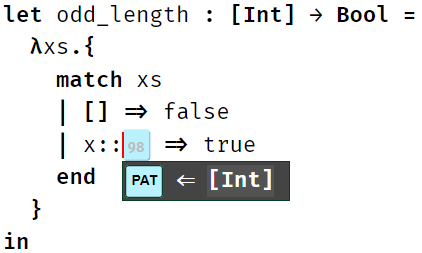
\includegraphics[scale=0.45,valign=t]{imgs/maybe_exhaustive.png}%
    \vphantom{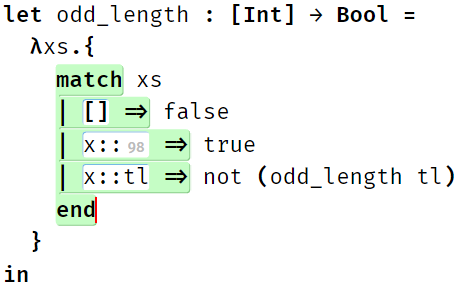
\includegraphics[scale=0.45,valign=t]{imgs/maybe_inexhaustive.png}}
}
\hfil
  \subfloat[Necessarily Inexhaustive\label{fig:not-exhautive}]{
    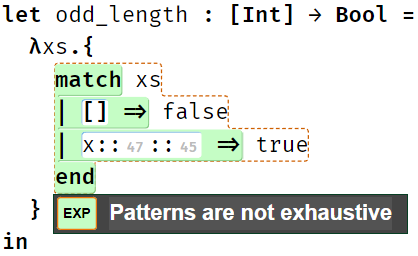
\includegraphics[scale=0.45,valign=t]{imgs/not_exhaustive.png}
    \vphantom{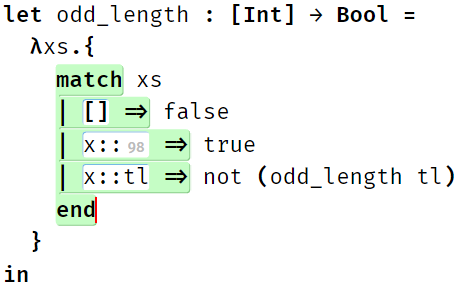
\includegraphics[scale=0.45,valign=t]{imgs/maybe_inexhaustive.png}}
}
\hfil
  \subfloat[Necessarily Exhaustive\label{fig:yes-inexhautive}]{
    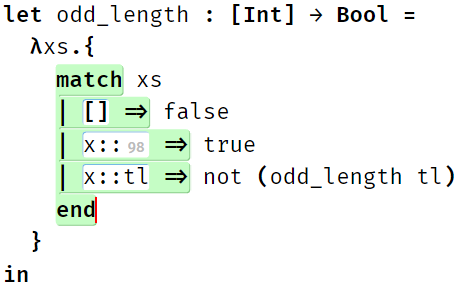
\includegraphics[scale=0.45,valign=t]{imgs/maybe_inexhaustive.png}
}
  \caption{Exhaustiveness Checking with Pattern Holes}
  \label{fig:exhaustiveness}
\end{figure}

We begin with the editor state in Fig.~\ref{fig:may-exhaustive}, 
where there is a hole in the tail position of the cons (\li{::}) pattern.
In determining whether this \li{match} expression is exhaustive, we 
must reason over all potential hole fillings. In this case, the 
\li{match} expression is \emph{indeterminately exhaustive}, because there are hole fillings,
such as a pattern variable \li{tl}, which would result in a determination
of exhaustiveness, while there are other hole fillings, such as \li{[]} or \li{y::tl},
where the determination would instead be inexhaustiveness. In the Hazel user interface, we choose to alert the programmer with an error
indicator only when the \li{match} expression is necessarily inexhaustive,
so no error appears for this editor state. The motivation for this choice is that we do not want to draw the programmer's attention for a problem that may or may not actually persist once the user has filled the holes. The cursor inspector does, however, provide typing information for the pattern hole when the programmer places their cursor there, as seen in Fig.~\ref{fig:may-exhaustive}. This and other pattern holes can be typed using information about how they are used. In this example, Hazel can determine that the pattern hole must have type \li{[Int]} because that is the only valid type for the right-hand side of the cons pattern when we are matching on \li{xs}, which is of type \li{[Int]}.

While pattern holes can make it impossible to conclusively determine the exhaustiveness of a \li{match} expression, the mere presence of a pattern hole does not mean that exhaustiveness errors never arise. Consider now
the editor state in Fig.~\ref{fig:not-exhautive}. In this case,
although there are again pattern holes in the second pattern, 
it can be determined that this \li{match} expression is \emph{necessarily inexhaustive}
because no matter how those holes are filled, this \li{match} expression will fail to 
match lists with exactly one element (singleton lists). Since this \li{match} expression is inexhaustive no matter how the holes are filled,
we alert the user with an error indicator and an error message when the cursor is on the \li{match} expression.


It is also possible for a \li{match} expression with pattern holes to be \emph{necessarily exhaustive}, as seen in Fig.~\ref{fig:yes-inexhautive}. Here, the first and third pattern are
exhaustive, regardless of how the hole in the second pattern is filled (e.g. with \li{[]} to special case singleton lists). We choose not to visually distinguish between necessarily and indeterminately exhaustive \li{match} expressions, again to avoid drawing
the programmer's attention to information that is unlikely to be actionable, but the
underlying semantic distinction is interesting to observe.

\subsection{Redundancy Checking with Pattern Holes}
\label{sec:hazel-redundancy}
A pattern is redundant if, for every value of the scrutinee's type that match that pattern, one of the preceding patterns in the \li{match} expression will necessarily 
match it. In the presence of pattern holes, we again have to consider all possible hole fillings in this analysis, leading to three possibilities: \emph{necessarily irredundant}, \emph{indeterminately irredundant}, and \emph{necessarily redundant} patterns.

In the editor state in Fig.~\ref{fig:may-redundant}, there is a pattern hole in the \emph{second} pattern of the \li{match} expression. It is possible to fill this hole in a way that would make the \emph{third} pattern irredundant, such as the empty list pattern, \texttt{[]}. 
However, it is also possible that the hole could be filled in a way that causes the third pattern to become redundant, such as the cons pattern \texttt{y::tl}. Consequently, the third pattern in this \li{match} expression is indeterminately irredundant (we chose ``irredundant'' rather than ``redundant'' in this phrase because, like exhaustiveness, irredundancy is the programmer's goal).

The second pattern itself, although it contains a pattern hole, is necessarily irredundant because no matter how the hole is filled, the first pattern, \li{[]}, does not overlap with it. The first pattern is always necessarily irredundant, even when it is a hole, because
there are no previous patterns (except if the scrutinee has the nullary sum, i.e. \li{void}, type, which has no values; see Supplementary Material).

The editor state in Fig.~\ref{fig:must-redundant} shows that a pattern with a hole can nevertheless be determined to be necessarily redundant.
In this case, the previous pattern handles every non-empty list, so no matter how the pattern hole is filled, it will be redundant.
Indeed, even an empty hole pattern in the third pattern would be redundant because the two preceding patterns are exhaustive.
 As with exhaustiveness, we only alert
the user to necessarily redundant patterns, so this is the only pattern in Fig.~\ref{fig:redundancy} where an error is reported.

\begin{figure}
    \begin{subfigure}[t]{0.45\textwidth}
    \centering
    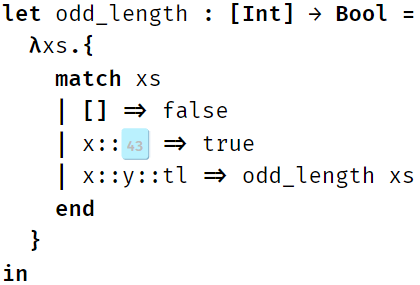
\includegraphics[scale=0.5,valign=t]{imgs/maybe_redundant.png}%
    \vphantom{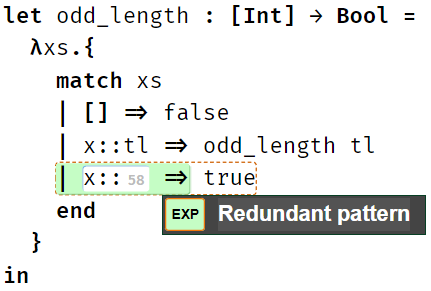
\includegraphics[scale=0.5,valign=t]{imgs/redundant.png}}
    \vspace{-6px}
    \caption{Necessarily Irredundant (first two patterns) + Indeterminately Irredundant (third pattern)\label{fig:may-redundant}}
    \end{subfigure}
    \begin{subfigure}[t]{0.45\textwidth}
    \centering
  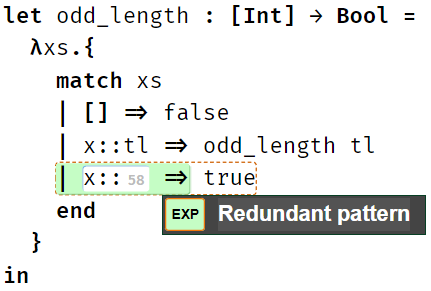
\includegraphics[scale=0.5,valign=t]{imgs/redundant.png}
  \vspace{-6px}
  \caption{Necessarily Redundant (third pattern) \label{fig:must-redundant}}
  \end{subfigure}
  \vspace{-3px}
  \caption{Redundancy Checking with Pattern Holes}
  \vspace{-3px}
  \label{fig:redundancy}
\end{figure}


\subsection{Live Evaluation with Expression and Pattern Holes}
\label{sec:hazel-live-eval}
In the examples above, we considered only {static analysis} of programs with pattern holes.
However, Hazel also supports live evaluation with holes, proceeding ``around'' holes
as necessary to produce a result with a possibly \emph{indeterminate value}, i.e. an expression that might retain holes in critical elimination positions \cite{DBLP:journals/pacmpl/OmarVCH19}.%\cite{DBLP:journals/tocl/NanevskiPP08}.

In a language without holes, the value of the scrutinee can be determined to either \emph{match} or \emph{mismatch} every pattern of the same type.
In order to support live evaluation with both expression and pattern holes, we have to consider now a third possiblilty: an \emph{indeterminate match} between the scrutinee, which may itself have an indeterminate value, and a pattern. Let us consider the possibilities in Fig.~\ref{fig:evaluation-ex}. 

We first look in Fig.~\ref{fig:exp-hole} at the situation where there are expression holes but no pattern holes. 
We see in \autoref{fig:exp-hole} that the argument to \li{odd_length} has a hole, so evaluation cannot determine a unique value. Instead,
the argument has an \emph{indeterminate value}. 
When we proceed through pattern matching, we can only make decisions that would be valid no matter how the hole in the tail of the list
would be filled. 
We can determine that the first pattern, \li{[]}, necessarily mismatches since the argument is not empty. 
Similarly, we can also determine that the second pattern necessarily mismatches because regardless of how the hole is filled, the list is at least of length two. 
When checking the third pattern, we see that this matches any list of at least two elements.
We know that the scrutinee necessarily matches this pattern, binding \li{tl} to whatever the hole is filled with, so we can take this branch. We next proceed to recurse, now with the hole itself as the argument. In the recursive call, we cannot determine whether the first pattern, \li{[]}, matches, since the empty expression hole could be filled with \li{[]} or with any other list. This indeterminate match leaves the entire \li{match} expression with an indeterminate value, and we cannot proceed any further as shown in the
evaluation result at the bottom of Fig.~\ref{fig:exp-hole}.

\begin{figure}
\begin{subfigure}[t]{0.45\textwidth}
\centering
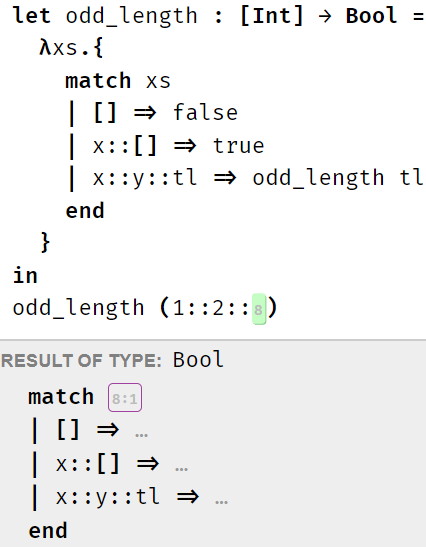
\includegraphics[scale=0.47,valign=t]{imgs/pat_match_exp_holes.png}\vphantom{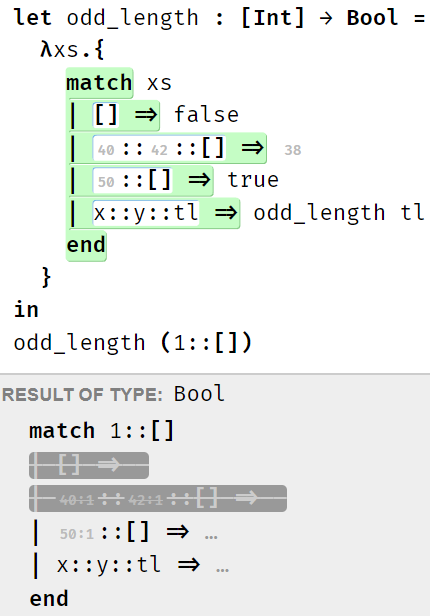
\includegraphics[scale=0.47,valign=t]{imgs/pat_match_pat_holes.png}}
\caption{Pattern matching with expression holes\label{fig:exp-hole}}
\end{subfigure}
\begin{subfigure}[t]{0.45\textwidth}
\centering
{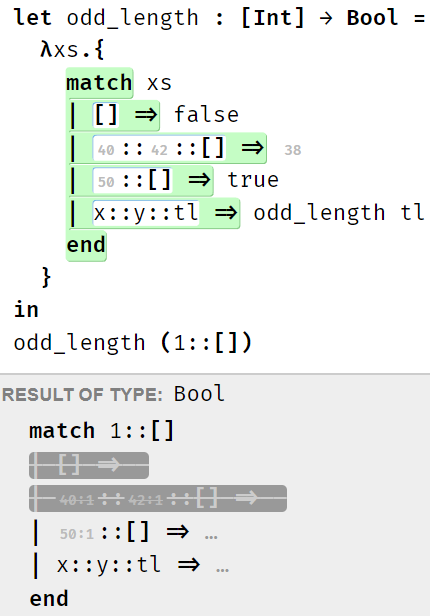
\includegraphics[scale=0.47,valign=t]{imgs/pat_match_pat_holes.png}}
\caption{Pattern matching with pattern holes\label{fig:pat-hole}}
\end{subfigure}
\vspace{-3px}
  \caption{Live Evaluation with Expression and Pattern Holes}
  \vspace{-3px}
  \label{fig:evaluation-ex}
\end{figure}


Next we consider in \autoref{fig:pat-hole} the situation where there are (several) pattern holes encountered during evaluation. 
We know that the first pattern, \li{[]}, necessarily mismatches the scrutinee, \li{1::[]}, for the standard reasons.
The second pattern, which contains two holes but which matches only lists of length two, also necessarily mismatches the scrutinee.
The third pattern matches singleton lists, like the scrutinee. However, a pattern hole appears at the pattern's head, so it cannot be determined 
whether there is necessarily a match or a mismatch with \li{1::[]}. For example, if the pattern hole is filled with the pattern \li{2}, 
then there would be a mismatch. Alternatively, if the pattern hole is filled with the pattern \li{x}, then there would be a match. This indeterminate match causes the \li{match} expression itself to have an indeterminate value.
However, by graying out mismatched rules in the result, we can report to the programmer how far match evaluation was able to proceed, as shown at the bottom of Fig.~\ref{fig:pat-hole}.